\documentclass[12pt,a4paper]{article}
\usepackage[top=25.4mm, bottom=25.4mm, left=19.1mm, right=19.1mm]{geometry}


\usepackage[latin2]{inputenc}
\usepackage{graphicx}
\graphicspath{ {./images/} }
\usepackage{ulem}
\usepackage{amsmath}
\usepackage[document]{ragged2e}

\setlength{\parindent}{4em}
\setlength{\parskip}{1em}
\usepackage{hyperref}

\usepackage{fancyhdr}
\pagestyle{fancy}
\fancyhf{}
\fancyhead[LO]{\textbf{\small IoT and Smart Analytics}\\
\text{\small A Program by IIITH and TalentSprint}}

\usepackage{xcolor}
\usepackage{lipsum}

\rhead{\begin{picture}(0,0) \put(-250,-2){
\includegraphics[width=9cm]{EXP_08_Images/ts-iisc-logo-pr.png}} \end{picture}}
\cfoot{\thepage}


\begin{document}

\begin{center}

\textbf{\large \\EXPERIMENT 11 }\\[6pt]
\text{Arduino Interfacing with Temperature, Humidity Sensor Module (GY-BME280), and LCD  }
\end{center}

\textbf{\large LEARNING OBJECTIVES:}\\[3pt]
At the end of this experiment, participants will be able to:\vspace{-6mm}\begin{enumerate}
\setlength\itemsep{-0.3em}
\item Connect & use Temperature, Humidity Sensor Module(GY-BME280)  with Arduino  \\
\item Connect & use LCD with Arduino \\ 
\item Understand & use I2C communication protocol in Arduino 
\end{enumerate}

\textbf{\large APPARATUS REQUIRED:}\\
\vspace{-3mm}
\begin{enumerate}
 \setlength\itemsep{-0.3em}
\item Arduino Module-1pcs \\
\item USB cable-1pcs\\
\item GY-BME280-1pcs\\
\item LCD(16X2)-1pcs\\
\item Resistor 10k$\Omega$ - 1pcs\\
\item Potentiometer-2pcs
\item Breadboard-1pcs\\
\item Jumper wires\\
\item Arduino IDE
\end{enumerate}

\begin{justify}
\textbf{\large THEORY}\\[3pt]
\textbf{A)	LCD (16X2): } In most electronic projects, we need a medium to display the output values (from a sensor) or some message. A Liquid Crystal Display,  commonly abbreviated as LCD is the best available option for such requirements, which comes in different size specifications. Out of all available LCD modules in the market, the most commonly used one is the 16×2 LCD Module, which can display 32 ASCII characters in 2 lines (16 characters in a line ). The module is based on the HD44780 driver (controller), having  16 pins, and can be operated in 4-bit mode (using only 4 data lines) or 8-bit mode (using all 8 data lines). The figure below shows a  16X2 LCD module with its pin naming.

\begin{center} 
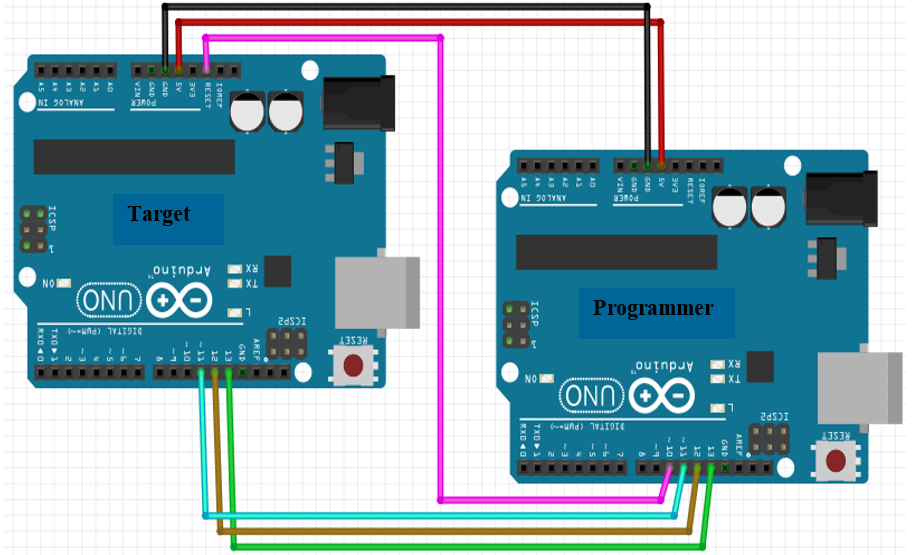
\includegraphics[scale=0.5]{EXP_11_Images/fig1.png}
\end{center}
\begin{center} {Figure 1. LCD (16X2) Module with pin naming}\end{center}

\noindent The functions of each pin of the module are given below: 

\noindent \textbf{Pin1(VSS):} Ground pin \\
\textbf{Pin2(VDD):} Power pin, +5V supply is given to this pin\\
\textbf{Pin3(V0): }Contrast adjustment pin. This is done by connecting the ends terminals of a 10K potentiometer to +5V and ground and then connecting the middle terminal (slider) to the V0 pin. The voltage at the V0 pin defines the contrast.\\
\textbf{Pin4(RS):} Register select pin. The module has two registers namely the data register and command register. Logic HIGH at RS pin selects data register and logic LOW at RS pin selects command register. \\
If we make the RS pin HIGH and feed input to the data lines (DB0 to DB7), this input will be treated as data to display on an LCD screen.\\
If we make the RS pin LOW and feed input to the data lines, then this will be treated as a command for LCD controller for tasks – like positioning cursor or clear screen or scroll.\\
\textbf{Pin5(RW):} Read/Write modes. Logic HIGH at this pin activates read mode and logic LOW at this pin activates write mode.\\
\textbf{Pin6(E):} This pin is meant for enabling the LCD module. A HIGH to LOW signal at this pin will enable the module.\\
\textbf{Pin7(D0) to Pin14(D7): }These are data pins. The commands and data are fed to the LCD module through these pins.\\
\textbf{Pin15(A):} Anode of the back light LED. \\
\textbf{Pin16(K):} Cathode of the back light LED.\\

\noindent \textbf{B) Temperature, Humidity Sensor Module(GY-BME280):  }
The BME280 sensor module reads barometric pressure, temperature, and humidity. We can also estimate altitude since pressure changes with altitude. There are several versions of this sensor module. The BME280 sensor uses I2C or SPI communication protocol to exchange data with a microcontroller.

\begin{center} 
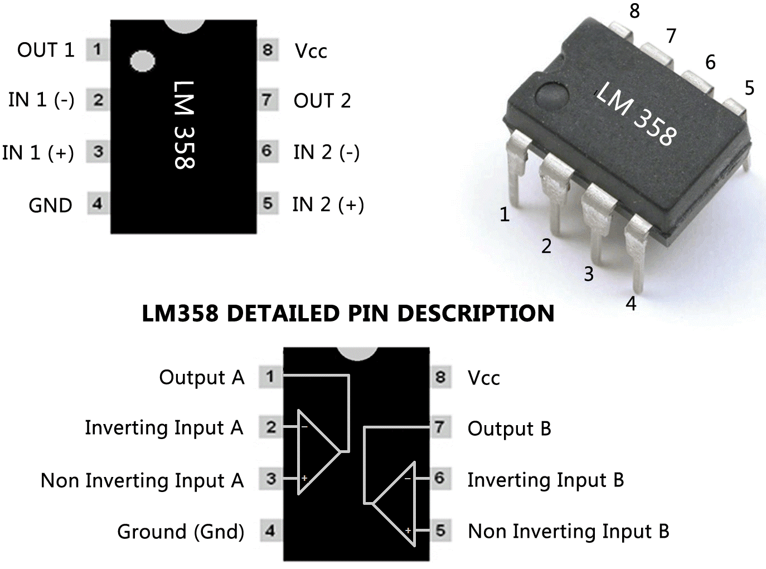
\includegraphics[scale=0.7]{EXP_11_Images/fig2.png}
\end{center}
\begin{center} {Figure 2. Six & four-pin versions of BME 280}\end{center}



\noindent Pin configuration for both versions is given in the table below. The Six-pin version may operate in both I2C and SPI communication protocols. While using BME280 with I2C communication SCK pin acts as SCL and SDI pin acts as SDA pin and leaves SDO and CS pin unconnected. \\
\vspace{20mm}
\begin{center} \textbf{Table 1. Pin configuration for two versions of  BME 280}\end{center}
\vspace{-5mm}
\begin{center} 
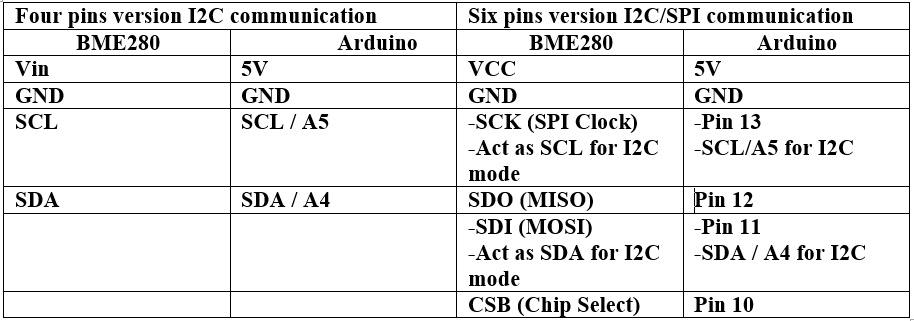
\includegraphics[scale=0.6]{EXP_11_Images/table.png}
\end{center}

\noindent \textbf{\large PROCEDURE}\\[3pt]
\textbf{A)	Interfacing LCD (16X2) with Arduino}\\[3pt]
\textbf{Hardware and software setup :} The RS pin of the LCD module is connected to digital pin 12 of the Arduino. RW pin of the LCD is grounded. Enable pin of the LCD module is connected to digital pin 11 of the Arduino. Here we are using the LCD module in 4-bit mode, i.e. only four of the digital input lines( D4 to D7) of the LCD are used. This is a simple way requiring fewer connections, and we can almost utilize the full potential of the LCD module. Digital lines D4, D5, D6, and D7 are interfaced to digital pins 5, 4, 3, and 2 of the Arduino. The 10K potentiometer is used for adjusting the contrast of the display. 10k ohm resistor limits the current through the back light LED. Another potentiometer is used to feed the analog signal to analog pin A0.


\begin{center} 
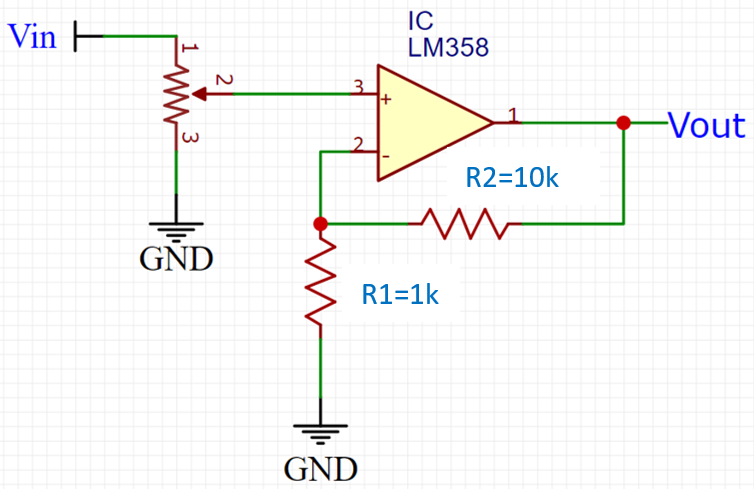
\includegraphics[scale=0.75]{EXP_11_Images/fig3.PNG}
\end{center}

\begin{center} {Figure 3. Interfacing LCD with Arduino}\end{center}

\noindent A built-in library in Arduino \textbf{$<L$iquidCrystal.h$>$}is used for communication between Arduino and LCD modules. This library can handle both 4-bit mode and 8-bit mode wiring of LCD. The library is readily available with the Arduino IDE (as it’s a pre-installed standard library).  Any library can be accessed manually through the \textbf{'Import library'} in the \textbf{'sketch'} tab in the main menu bar.
In the following program, we want to display the analog read value available on analog pin A0 and the time elapsed since Arduino is triggered in the second line along with the msg 'IoT Learning' in the first line. \end{justify}

\hspace{2cm}\textbf{\large Code:}\\[6pt]


\setlength{\parindent}{10eM}

\##include $<$LiquidCrystal.h$>$  \textcolor{blue}{// include the library code:\\
// initialize the library by associating any needed LCD interface/ \\ Arduino pin}\\

const int rs = 12; en = 11; d4 = 5; d5 = 4; d6 = 3; d7 = 2;\\
LiquidCrystal lcd(rs, en, d4, d5, d6, d7);\\

void setup()\\ 
\{\\	
\textcolor{blue}{// set up the LCD's number of columns and rows:}\\
lcd.begin(16, 2);\\
\textcolor{blue}{// Print a message to the LCD.}\\
lcd.print("IoT Learning!");\\
\}

void loop() \\
\{  \\ 
  int value=analogRead(A0);\\

   if(value $<$ 1000)\\
  \{ lcd.setCursor(3, 1);\\
    lcd.print(" "); \}\\

  \textcolor{blue}{// set the cursor to column 0, line 1}\\
  \textcolor{blue}{// (note: line 1 is the second row, since counting begins with 0):}\\
  lcd.setCursor(0, 1);\\
  lcd.print(value);\\
 \textcolor{blue}{// print the number of seconds since reset:}\\
  lcd.setCursor(7, 1);\\
  lcd.print(millis() / 1000);\\

\}

\setlength{\parindent}{0pt}

\begin{justify} \noindent \underline {\textbf{Explanation of LCD functions used in the code:}}\\[9pt]
\noindent \textbf{LiquidCrystal lcd() } is  a constructor used to declare an object ‘lcd’ of class  ‘LiquidCrystal.h’. Here 'lcd' is used to invoke methods defined inside the 'LiquidCrystal.h' class (Example– lcd.print(); lcd.setCursor() and other methods). LCD interfacing pins  with Arduino pins are passed as variables (here defined as contants).\\
\textbf{lcd.begin()}\– is called to initialize the lcd screen and to pass the dimension of the lcd screen (columns, rows) as parameters of the invoked method.\\
\textbf{lcd.print('msg')}\- Print \"msg\" to the LCD.\\
\textbf{lcd.setCursor(c,r)}\- set the cursor to column \‘c\’, and row (line) \‘r\’. By default cursor is at zeroth row and zeroth column.


\noindent \textbf{B) Interfacing Sensor Module(GY-BME280) with Arduino}\\[3pt]
\textbf{Hardware and software setup :}In this example, SPI protocol is used and pins are connected as given in table1. The I2C communication protocol can also be used with an appropriate pin connection. To get readings from the BME280 sensor module, we need to use the Adafruit\_BME280 library. This library can be searched in Arduino IDE by going to \textbf{Sketch $>$ Include Library $>$ Manage Libraries}. Search for \textbf{'adafruit bme280 '} in \textbf{Library Manager} on the Search box and install the library.\end{justify}


\begin{center} 
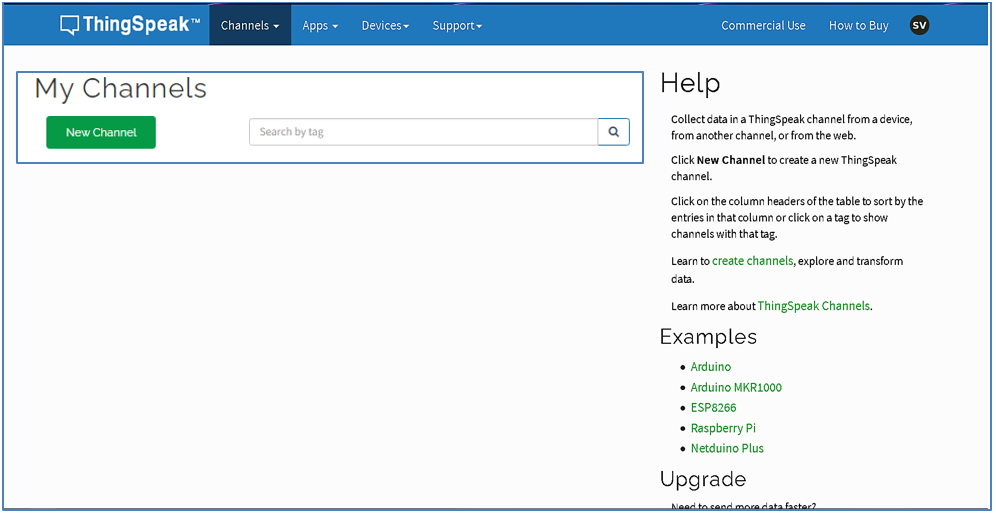
\includegraphics[scale=0.7]{EXP_11_Images/fig4.png}
\end{center}
\begin{center} {Figure 4. Interfacing BME280 sensor with Arduino using SPI protocol}\end{center}

\hspace{1.7cm}\textbf{\large Code:}\\[6pt]
\setlength{\parindent}{7eM}

\textcolor{blue}{//\#include $<$Wire.h$>$ // this library is used for I2C protocol,commented here}\\
\#include $<$SPI.h$>$ \textcolor{blue}{// used for SPI protocol, comment this for I2C}\\
\textcolor{blue}{// Following two libraries are used tor interfacing with BME280 sensor}\\
#include $<$Adafruit\_Sensor.h$>$\\
#include $<$Adafruit\_BME280.h$>$\\
\textcolor{blue}{// Following are the pin configuration for SPI\\
// Not used for I2C}\\
\#define BME\_SCK 13   \textcolor{blue}{//SPI} \\
\#define BME\_MISO 12  \textcolor{blue}{//SDO}  \\
\#define BME\_MOSI 11 \textcolor{blue}{ //SDI } \\
\#define BME\_CSB 10 \\
\#define SEALEVELPRESSURE\_HPA (1013.25)\\

\textcolor{blue}{//Adafruit\_BME280 bme; //used for I2C, commented here}\\
Adafruit\_BME280 bme(BME\_CSB, BME\_MOSI, BME\_MISO, BME\_SCK);\\ 
\textcolor{blue}{//for SPI only, not used in I2C}\\
unsigned long delayTime;\\[13pt]

void setup()\\
\{\\
Serial.begin(9600); \textcolor{blue}{// serial communication started}\\
    while(!Serial);   \textcolor{blue} { // time to get serial running}\\
    Serial.println(F("BME280 test"));\\

    unsigned status;\\
    status = bme.begin(); \textcolor{blue}{//sensor is initialized using SPI \\ 
    //status = bme.begin(0x76); / /sensor is initialized using I2C}\\

     if (!status)\\
     \{\\
Serial.println("No any valid BME280 sensor\\ available.Something is wrong.Please      check!");\\
  while (1);\\
     \}\\
    delayTime = 1000;\\
    Serial.println();\\

\}\\[13pt]

void loop()\\
\{\\
printValues();\\
delay(delayTime);\\
\}\\[21pt]

\textcolor{blue} {/*  In the loop(), the printValues() function reads the values from the BME280\\ 
   print the results in the Serial Monitor.*/}\\[15pt]

void printValues() \\
\{\\
    Serial.print("Temperature = ");\\
    Serial.print(bme.readTemperature());\\

Serial.println(" $^{\circ}$ C");\\

    Serial.print("Pressure = ");\\
    Serial.print(bme.readPressure() / 100.0F);\\
    Serial.println(" hPa");\\

    Serial.print("Approx. Altitude = ");\\
    Serial.print(bme.readAltitude(SEALEVELPRESSURE\_HPA));\\
    Serial.println(" m");\\

    Serial.print("Humidity = ");\\
    Serial.print(bme.readHumidity());\\
    Serial.println(" \%");\\
    Serial.println();\\

    \}\\



\begin{justify} Note: A variable named 'SEALEVELPRESSURE\_HPA' is defined which, saves the pressure at the sea level in hectopascal (100x multiple of the Pascal). This variable is used to estimate the altitude for a given pressure by comparing it with the sea level pressure. Here we have used the default value, but for more accurate results, replace the value with the current sea level pressure at your location.

\setlength{\parindent}{0eM}

\textbf{\large CONCEPT DRILLS:}
\vspace{-6mm}
\begin{enumerate}
 \setlength\itemsep{-0.3em}
\item Design a circuit and write the appropriate program to interface LCD and BME280 sensor so that we can get readings of temperature and pressure in LCD screen as shown in the figure below.


\begin{center} 
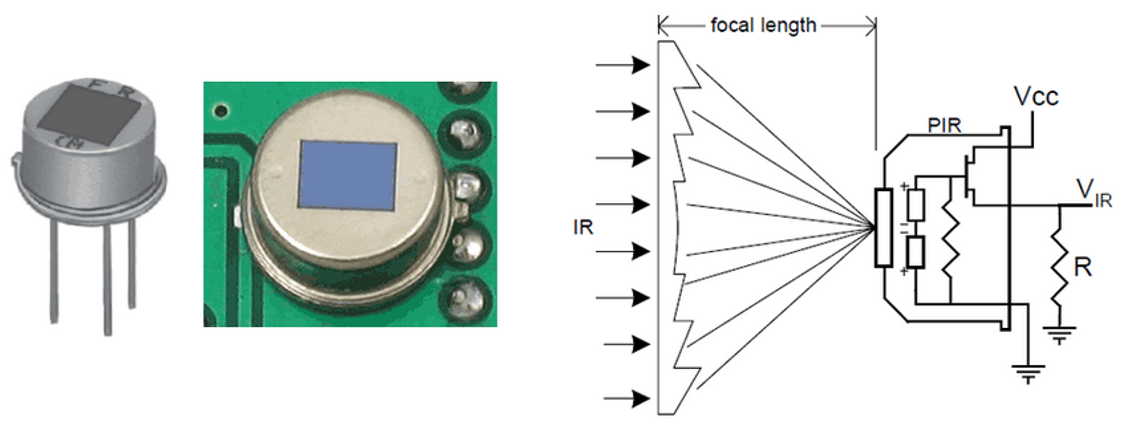
\includegraphics[scale=0.55]{EXP_11_Images/fig5.png}
\end{center}
\begin{center} {Figure 5. Sensor value display in LCD screen}\end{center}
\end{enumerate}
\end{justify}
\end{document}